%\setlength\abovedisplayskip{2.5pt}

For relevant nuclear forensics predictions, both classification and regression
algorithms must be used.  For example, one may want to predict the reactor type
label given some measurement-based features of \gls{SNF} of an unknown source.
This would require a classification algorithm. Or perhaps the input fuel
composition is relevant to an investigation on weapons intent, so a regression
algorithm would be used. 

To limit the scope of this work, it cannot be an exhaustive study of \gls{ML}
methods.  Therefore, three algorithms are presented in this section:
\textit{k}-nearest neighbors, decision trees, and \gls{MLL} calculations. They
were chosen based on their simplicity; this work has yet to be benchmarked
using simple algorithms so a more complex treatment of the training sets in
this work would be premature. Additionally, in part because of their
simplicity, they are all "white box" methods.  This is unique in the \gls{ML}
universe, since most algorithms create a black box model that is unable to be
analyzed by a human.  The  decision trees method provides an output model that
can be used to discern behavior and understand predictions, and
\textit{k}-nearest neighbors and \gls{MLL} calculations do not create a model
at all. Individual predictions can still be analyzed, however, since the
procedures are so simple. 

\subsubsection{Nearest Neighbors}

Nearest neighbors classification and regression are unique algorithms in
that they are instance-based; they do not actually generalize, but instead
track the observations in the training set.  The main metric for this algorithm
is distance (or dissimilarity) between the test sample and the closest training
sample(s) in the vicinity.  During prediction, the algorithm will calculate a
value based on the instance that is closest to the current test sample. Thus,
there is not any learning, but instead a direct comparison between an unknown
sample and the space that the training set populates. The predictions from
nearest neighbors can be quite accurate, but are highly unstable to
perturbations \cite{elements_stats}.

The process of prediction with \textit{k}-nearest neighbors is as follows.
First, the distances between the test sample and each of the training set
instances are calculated.  Most commonly the Euclidean distance is used, but
this walk-through uses the Manhattan distance:
\begin{equation}
  d_{i} = \sum_{j=1}^{N_{feats}} |x_{j,train} - x_{j,test}|
  \label{eq:l1}
\end{equation}
where $i$ is each training set instance, and $j$ refers to each feature in the
training set.  The lowest \textit{k} $d_{i}$ are chosen. For \textit{k}-nearest
neighbors regression, the value, $y$ is predicted using the following equation.
\begin{equation}
  y(\boldsymbol{x}) = \frac{1}{\sum_{i}{w_i}} \sum_{i=1}^{k} w_i \cdot y_i
  \label{eq:knn}
\end{equation}
where $w_{i}$ is either uniform and takes on a value of $1$ or is
distance-based and takes on a value of $1/d_{i}$ and $\boldsymbol{x}$ is the
full set of features. The regression equation averages the closest \textit{k}
neighbors for an estimate of the unknown sample.  In \textit{k}-nearest
neighbors classification, the class label $y$ is predicted using the mode of
the nearest neighbors selected using the \textit{k} smallest $d_i$, or when
$w_i$ is $1/d_i$, the weighted mode is used to choose the predicted label.

\begin{figure}[!htb]
  \centering
  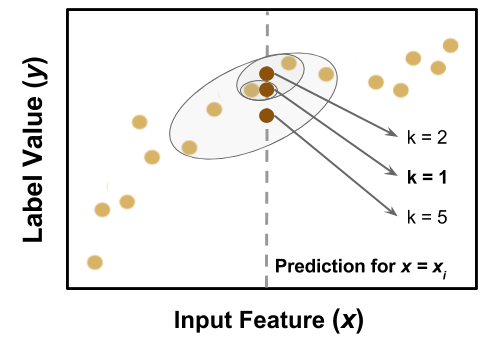
\includegraphics[width=0.8\linewidth]{./chapters/litrev/nn-fig.png}
  \caption[Schematic of \textit{k}-nearest neighbors regression]
          {Schematic of \textit{k}-nearest neighbors regression, showing how 
           changing \textit{k} alters the predicted label value $y$.}
  \label{fig:nn}
\end{figure}

Figure \ref{fig:nn} provides a pictorial explanation of Equation \ref{eq:knn}
for a prediction where there is one feature. In this figure, there is a test
sample with a feature, valued at $x_i$, indicated with the grey dotted line.
The three circles represent the neighborhood given by the value of \textit{k},
and the darker dots on the line represent the reported prediction $y$ for each
choice of \textit{k}.  In this illustration, $k=1$ or $k=2$ provide a more
accurate prediction according to a visual inspection of the trend, but higher
values of $k$ can be useful, and will be discussed in Section
\ref{sec:complexity}.

\subsubsection{Decision Trees}

Decision trees are a common choice because they are simple to implement and
provide an interpretable model. However, the predictions from decision trees,
similar to \textit{k}-nearest neighbors, are unstable to perturbations.  What
follows is a highly simplified explanation of the Classification and Regression
Trees algorithm for growing decision trees, showing only the equations for
splitting criteria.  A more complete treatment can be found in Reference
\cite{elements_stats} or in the User Guide in Reference \cite{scikit}.

At their core, decision trees algorithms split the feature space into different
regions.  Decision trees are constructed by iteratively finding places in the
feature space at which to split the data to best predict a label. Some measure
of information gain (more accurately the opposite, impurity, denoted here as
$H$ is used to select a splitting criterion at each split, which maximizes
differentiation between average label values in regression or groups similar
labels together in classification.  This process continues until some
externally set stopping requirement is met, or no information gain can be made
by continuing to create splits. 

Each split creates two new nodes on the tree, where the node has to find a new
splitting criterion. In the math that follows, there are nodes given by $m$,
and a number of samples in each node given by $N_{\text{samples}, m}$. The
individual node samples are counted by $i$, and so the sample labels are $y_i$.
The impurity at the node is denoted as $H(m)$.  In classification, the node
impurity $H(m)$ can be measured by the Gini index, where $p_{m, k}$ is the
proportion of class $k$ observations at the node:
\begin{equation}
  \begin{aligned}
    p_{m, k} &= \frac{1}{N_{\text{samples}, m}} \sum_{i=1}^{N_{\text{samples}, m}}
                \mathbb{I}(y_i = k)
    \\
    H(m) &= \sum_k p_{m, k} (1 - p_{m, k})
  \end{aligned}
  \label{eq:gini}
\end{equation}
Note that $\mathbb{I}()$ here is being used to refer to the indicator function,
where when $y=k$ it takes a value of 1 and when $y \neq k$ it takes a value of 0.
And in regression, the node impurity $H(m)$ can be measured by the mean squared
error, where $\bar{y}_m$ is the average value of the samples in the node.
\begin{equation}
  \begin{aligned}
    \bar{y}_m &= \frac{1}{N_{\text{samples}, m}} \sum_{i=1}^{N_{\text{samples}, m}} 
                 y_{i, m}
    \\
    H(m) &= \frac{1}{N_{\text{samples}, m}} \sum_{i=1}^{N_{\text{samples}, m}}
            (y_i - \bar{y}_{i, m})^2
  \end{aligned}
  \label{eq:mse}
\end{equation}
The splitting criterion with the lowest impurity is the one that is chosen to
make the split.  This will partition the feature space and the splitting
process will continue until a pre-defined tree size or number of samples per
node. Without a pre-defined stopping point the tree will grow until there is
one sample per node. This process can be understood more intuitively by
studying Figure \ref{fig:dtr}. Note that this tree was created using a maximum
tree depth of $3$ for visualization purposes in order to explain the process,
so is not indicative of a real decision tree.

\begin{figure}[!htb]
  \centering
  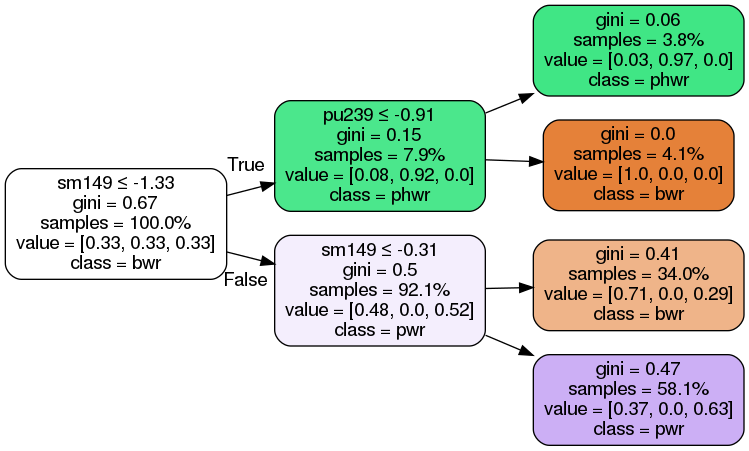
\includegraphics[width=\linewidth]{./chapters/litrev/dtree.png}
  \caption[Example of a decision tree]
          {Example of a decision tree process, where maximum tree depth is 
           limited to 3.}
  \label{fig:dtr}
\end{figure}

In Figure \ref{fig:dtr}, each node has the following information: the splitting
criterion, Gini impurity value, percentage of samples in the training set in
the node, a value list (explained below), and the majority class present in the
node.  In the visualization, the shading of the colors in the tree are bolder
for there being a higher fraction of a single class. As a method that produces
a model that can be understood by humans, the reasoning for the splits is also
discussed.

The first split is determined to occur at the feature ${}^{149}\text{Sm}$ on
whether the nuclide measurement is above or below a value of $-1.33$. Note that
this value is negative because of the scaling process the training set is put
through, described in Section \ref{sec:statmodel1}. This is an unsurprising
split because the creation of ${}^{149}\text{Sm}$ is heavily dependent on the
neutron energy spectrum and thus helps distinguish reactor types. The majority
class at this node is \gls{BWR} which is expected since the training set is
72\% \gls{BWR}.  The values list indicates the fraction of each class in the
node, which is alphabetically ordered by \texttt{[BWR, PHWR, PWR]}. It is even
among the three because the class weights are balanced.  This splitting
criterion provides a Gini impurity score of 0.67, which represents the minimum
Gini impurity of all the candidate splits, but also indicates there are
multiple classes represented in this node (again, expected).  It would be 0 if
there were only one class in the node.  

The next level of the decision tree in Figure \ref{fig:dtr} has two nodes. The
top node has a splitting criterion of whether ${}^{239}\text{Pu}$ is above or
below a value of $-0.91$.  This is also an unsurprising choice for the decision
tree because its creation and destruction is heavily dependent on the enrichment,
since \glspl{PHWR} have more ${}^{238}\text{U}$ available for neutron capture.
This node contains a majority of the \gls{PHWR} class, but also a fraction of
0.08 of the \gls{BWR} class.  Even though the \gls{PHWR} class is only 1.5\% of
the training set (see Section \ref{sec:training1}), this node has 7.9\% of the
training set samples.  The next level split for the top node has fractions of
0.97 \gls{PHWR} and 1.0 \gls{BWR} in the next two nodes, with Gini impurities
of 0.06 and 0.0, respectively. This is a rapid approach to zero considering the
size of the training set and number of features. 

The lower node has a splitting criterion of whether ${}^{242m}\text{Am}$ is
above or below 0.68.  This one is less obvious of a choice, but is in the decay
chain of ${}^{241}\text{Pu}$ (if it does not fission), which is created by a
series of neutron captures.  This links ${}^{242m}\text{Am}$ to a dependence on
the neutron energy spectrum and therefore makes it somewhat capable of
distinguishing reactor type.  The remaining 92.1\% of the training set is in
this node, and there is only a slight majority of the (balanced) \gls{PWR}
class, which is why the shading is nearly white. The Gini impurity for the top
node is 0.15.  This is much lower than the Gini impurity of 0.5 for the bottom
node, which is more evenly split between two classes.  The next level split for
the bottom node made modest improvements over the Gini impurity of 0.5, and
would need to go much deeper to properly classify \gls{PWR} versus \gls{BWR}.
This suggests that ${}^{242m}\text{Am}$ is only a moderate reactor type
indicator.

\subsubsection{Maximum Log-Likelihood Calculations}

The \gls{MLL} calculations approach applied here is based on a method developed
to do similar work \cite{mll_method, mll_validate, mll_sensitivity}.  That work
involved matching nuclear material samples based on some select measurements to
entries in a database of containing those measurements (see Section
\ref{sec:stats4nf}).  Each database entry also has a similar list of labels to
the labels being predicted in this work: reactor type, burnup, and time since
irradiation.

Interestingly, the \gls{MLL} calculations method works exactly like
\textit{k}-nearest neighbors with $k=1$, where there is no model but a
prediction according to the closest match database entry.  There is one detail
that differs, however: the selection criterion.  Whereas \textit{k}-nearest
neighbors minimizes distance/dissimilarity, this approach instead maximizes
similarity via a likelihood function. An "unknown" test sample is compared
against the training set using the likelihood calculation between that sample
and the training set entries.  The higher the likelihood, the higher the
probability that the database entry represents the sample. The likelihood is in
Equation \ref{eq:like}, whereas the log-likelihood is used more often in
practice, shown in Equation \ref{eq:loglike} \cite{mll_method}.
\begin{equation}
  L(M|x_{test}) = \prod_i \frac{1}{\sigma_{i,train} \sqrt{2\pi}} \exp{\frac{-(x_{i,test} - x_{i,train})^2}{2 \sigma_{i,train}^2}}
  \label{eq:like}
\end{equation}
\begin{equation}
  ln(L(M|x_{test})) = \sum_i ln(\frac{1}{\sigma_{i,train} \sqrt{2\pi}}) - \frac{(x_{i,test} - x_{i,train})^2}{2 \sigma_{i,train}^2}
  \label{eq:loglike}
\end{equation}
Although these equations were borrowed directly from Reference
\cite{mll_method}, some of the variables have been changed for better cohesion
with the terminology in this work.  The likelihood is a measure of the
probability that a model $M$ produced the measurements seen in the test sample,
given by $L(M|x_{test})$.  In both Equations \ref{eq:like} and
\ref{eq:loglike}, $x$ refers to the set of features, and $x_{i, test}$ and
$x_{i,train}$ are the individual features for the test sample and the training
set entries, respectively. The uncertainty of the measurement associated with
each feature is represented by $\sigma_{i,train}$.

